%%
%% This is file `sample-sigplan.tex',
%% generated with the docstrip utility.
%%
%% The original source files were:
%%
%% samples.dtx  (with options: `sigplan')
%% 
%% IMPORTANT NOTICE:
%% 
%% For the copyright see the source file.
%% 
%% Any modified versions of this file must be renamed
%% with new filenames distinct from sample-sigplan.tex.
%% 
%% For distribution of the original source see the terms
%% for copying and modification in the file samples.dtx.
%% 
%% This generated file may be distributed as long as the
%% original source files, as listed above, are part of the
%% same distribution. (The sources need not necessarily be
%% in the same archive or directory.)
%%
%% The first command in your LaTeX source must be the \documentclass command.
\documentclass[sigplan,screen]{acmart}
%% NOTE that a single column version is required for 
%% submission and peer review. This can be done by changing
%% the \doucmentclass[...]{acmart} in this template to 
%% \documentclass[manuscript,screen,review]{acmart}
%% 
%% To ensure 100% compatibility, please check the white list of
%% approved LaTeX packages to be used with the Master Article Template at
%% https://www.acm.org/publications/taps/whitelist-of-latex-packages 
%% before creating your document. The white list page provides 
%% information on how to submit additional LaTeX packages for 
%% review and adoption.
%% Fonts used in the template cannot be substituted; margin 
%% adjustments are not allowed.
%%
%% \BibTeX command to typeset BibTeX logo in the docs
\AtBeginDocument{%
  \providecommand\BibTeX{{%
    \normalfont B\kern-0.5em{\scshape i\kern-0.25em b}\kern-0.8em\TeX}}}

%% Rights management information.  This information is sent to you
%% when you complete the rights form.  These commands have SAMPLE
%% values in them; it is your responsibility as an author to replace
%% the commands and values with those provided to you when you
%% complete the rights form.
% \setcopyright{acmcopyright}
% \copyrightyear{2018}
% \acmYear{2018}
% \acmDOI{10.1145/1122445.1122456}

%% These commands are for a PROCEEDINGS abstract or paper.
% \acmConference[Woodstock '18]{Woodstock '18: ACM Symposium on Neural
%   Gaze Detection}{June 03--05, 2018}{Woodstock, NY}
% \acmBooktitle{Woodstock '18: ACM Symposium on Neural Gaze Detection,
%   June 03--05, 2018, Woodstock, NY}
% \acmPrice{15.00}
% \acmISBN{978-1-4503-XXXX-X/18/06}


%%
%% Submission ID.
%% Use this when submitting an article to a sponsored event. You'll
%% receive a unique submission ID from the organizers
%% of the event, and this ID should be used as the parameter to this command.
%%\acmSubmissionID{123-A56-BU3}

%%
%% The majority of ACM publications use numbered citations and
%% references.  The command \citestyle{authoryear} switches to the
%% "author year" style.
%%
%% If you are preparing content for an event
%% sponsored by ACM SIGGRAPH, you must use the "author year" style of
%% citations and references.
%% Uncommenting
%% the next command will enable that style.
%%\citestyle{acmauthoryear}

%%
%% end of the preamble, start of the body of the document source.
\setcopyright{none}
\settopmatter{printacmref=false}
\begin{document}

%%
%% The "title" command has an optional parameter,
%% allowing the author to define a "short title" to be used in page headers.
\title{MoReBergers: Social Media Prediction}

%%
%% The "author" command and its associated commands are used to define
%% the authors and their affiliations.
%% Of note is the shared affiliation of the first two authors, and the
%% "authornote" and "authornotemark" commands
%% used to denote shared contribution to the research.
\author{Mohamed Kleit}
\email{mohamed.kleit@umontreal.ca}
\affiliation{%
  \institution{Université de Montréal}
}

\author{Lucia Eve Berger}
\email{lucia.eve.berger@umontreal.ca}
\affiliation{%
  \institution{Université de Montréal}
}

\author{Alireza  Razaghi}
\email{alireza.razaghi@umontreal.ca}
\affiliation{%
  \institution{Université de Montréal}
}
%%
%% By default, the full list of authors will be used in the page
%% headers. Often, this list is too long, and will overlap
%% other information printed in the page headers. This command allows
%% the author to define a more concise list
%% of authors' names for this purpose.
%\renewcommand{\shortauthors}{Trovato and Tobin, et al.}

%%
%% The abstract is a short summary of the work to be presented in the
%% article.
\begin{abstract}
In this report, we present the analysis and results obtained as part of a Kaggle competition on social media prediction. We developed a model capable of accurately predicting the number of profile likes based on simulated social media profile information. We followed an iterative process with an embedded feedback-loop between the data preprocessing, model selection and model performance. 

Through our process, we developed two models which provided our best performances on the private test set: an ensemble of gradient boosting models and a multi-layer Neural Network. With the former, we obtained a Root Mean Squared Logarithmic Error (RMSLE) of 1.6719 and a RMSLE of 1.6712 on the latter.
\end{abstract}

%%
%% The code below is generated by the tool at http://dl.acm.org/ccs.cfm.
%% Please copy and paste the code instead of the example below.
%%
% \begin{CCSXML}
% <ccs2012>
%  <concept>
%   <concept_id>10010520.10010553.10010562</concept_id>
%   <concept_desc>Computer systems organization~Embedded systems</concept_desc>
%   <concept_significance>500</concept_significance>
%  </concept>
%  <concept>
%   <concept_id>10010520.10010575.10010755</concept_id>
%   <concept_desc>Computer systems organization~Redundancy</concept_desc>
%   <concept_significance>300</concept_significance>
%  </concept>
%  <concept>
%   <concept_id>10010520.10010553.10010554</concept_id>
%   <concept_desc>Computer systems organization~Robotics</concept_desc>
%   <concept_significance>100</concept_significance>
%  </concept>
%  <concept>
%   <concept_id>10003033.10003083.10003095</concept_id>
%   <concept_desc>Networks~Network reliability</concept_desc>
%   <concept_significance>100</concept_significance>
%  </concept>
% </ccs2012>
% \end{CCSXML}

% \ccsdesc[500]{Computer systems organization~Embedded systems}
% \ccsdesc[300]{Computer systems organization~Redundancy}
% \ccsdesc{Computer systems organization~Robotics}
% \ccsdesc[100]{Networks~Network reliability}

%%
%% Keywords. The author(s) should pick words that accurately describe
%% the work being presented. Separate the keywords with commas.
% \keywords{social media, RMSLE, gradient boosting, multi-layer perceptron, kaggle, preprocessing}

%% A "teaser" image appears between the author and affiliation
%% information and the body of the document, and typically spans the
%% page.
% \begin{teaserfigure}
%   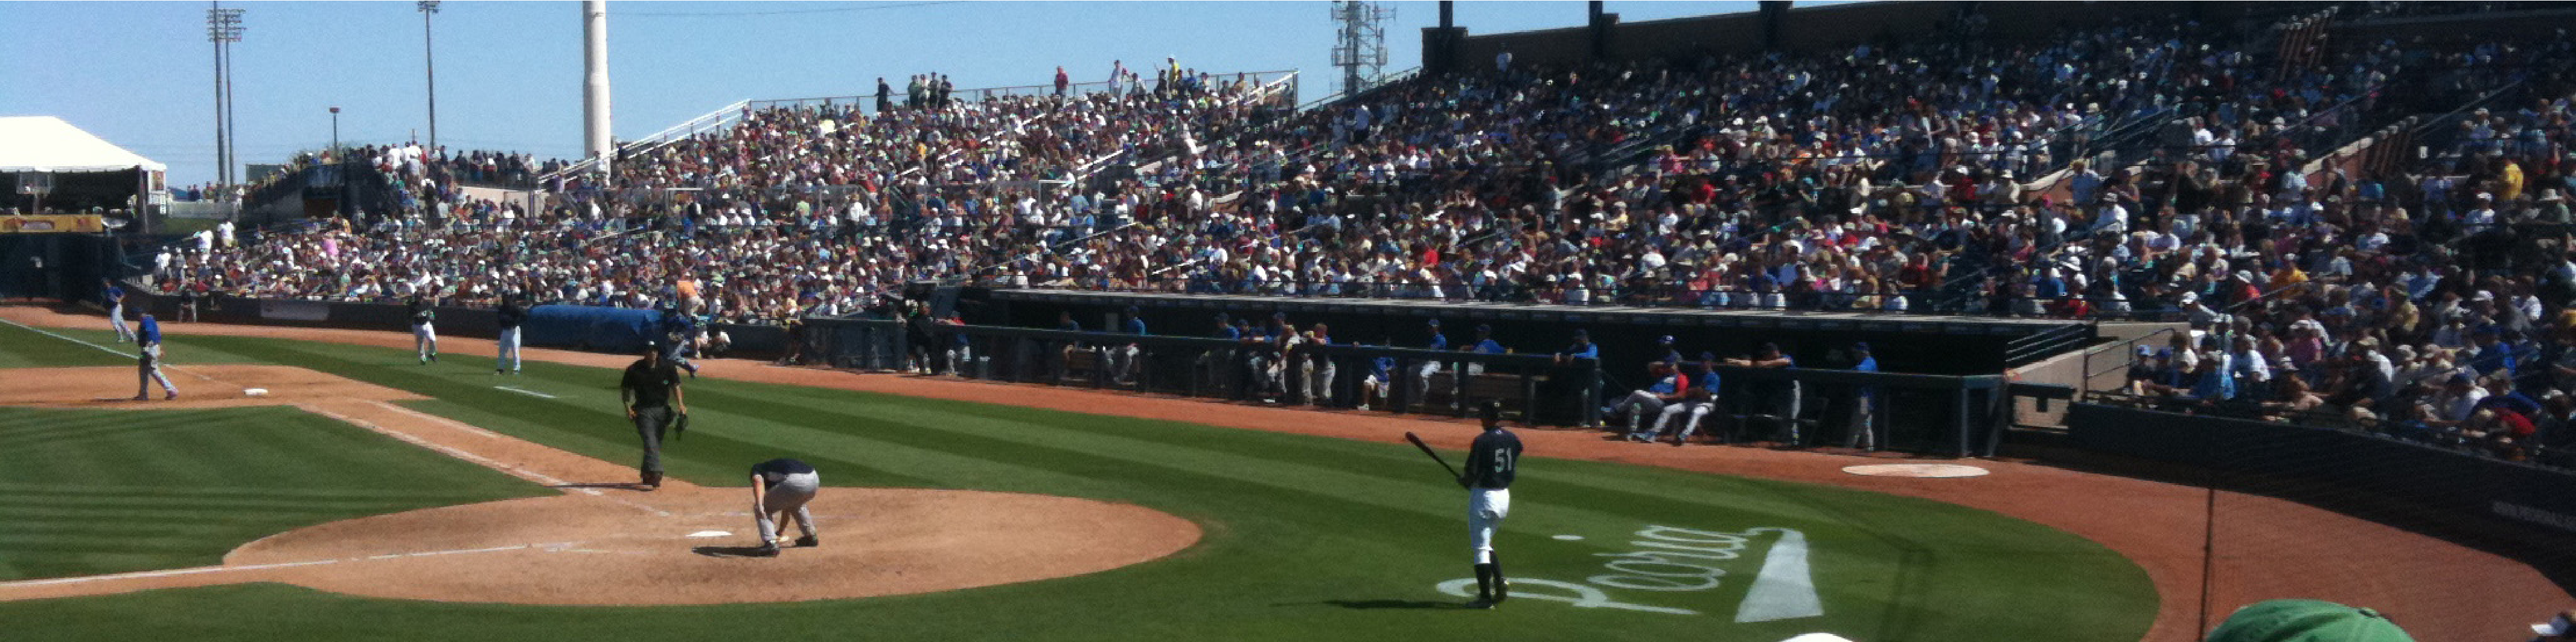
\includegraphics[width=\textwidth]{sampleteaser}
%   \caption{Seattle Mariners at Spring Training, 2010.}
%   \Description{Enjoying the baseball game from the third-base
%   seats. Ichiro Suzuki preparing to bat.}
%   \label{fig:teaser}
% \end{teaserfigure}

%%
%% This command processes the author and affiliation and title
%% information and builds the first part of the formatted document.
\maketitle

\section{Introduction}
In this competition, we were tasked with predicting  the number of profile likes. This can be understood as a supervised regression problem. The train dataset provided included 7500 observations and 24 features (23 features, 1 label). The test dataset includes 2500 observations.  

\section{Data Cleaning}
The first part of any machine learning or data science project is data cleaning. Data cleaning is the process of detecting and correcting (or removing) corrupt or inaccurate records from a record set, table, or database and refers to identifying incomplete, incorrect, inaccurate or irrelevant parts of the data and then replacing, modifying, or deleting the dirty or coarse data.[Wikipedia]

\subsection{Addressing Missing values}

As seen in Figure \ref{addressing_missing_values}, we encountered missing values in different features.  For each one, we took a different approach. Our approaches can be classified as below:
\begin{itemize}
    \item 
    \textbf{Numerical columns:}
    For \textit{'Avg Daily Profile Clicks'} and \textit{'Avg Daily Profile Visit Duration in seconds'} columns, we used mean imputation. We used SimpleImputer from sklearn and replaced all the missing values with the mean value of that feature.
    \item
    \textbf{Categorical columns:}
    \begin{itemize}
        \item 
        For \textit{‘Personal URL’} and \textit{‘Profile Cover Image Status’} columns we simply replaced missing values with 0 and also replaced all other values with 1. Thus, at the end we have a column with either 0 or 1.
        \item
        For \textit{‘Profile Theme Color’}, \textit{‘Profile Text Color'}, \textit{‘Profile Page Color’}, \textit{‘UTC offset’}, and\textit{ ‘User Time Zone’}, we replaced the missing values with the most frequent value in the column.
        \item
        For the \textit{‘Profile Category’} column, first the white spaces were replaced by NaN values and then the Nan values were replaced by \textit{‘Unknown'}.
    \end{itemize}
\end{itemize}

\subsection{Removed Features}
After carefully investigating all the features we decided to remove few of them. First \textit{'ID'} and \textit{'Username'} columns are irrelevant to our target. The Location column was very messy and also we could extract a sense of location from other columns such as User Time Zone. So we dropped the Location. Finally, we decided to drop the \textit{'Profile Image'} column because of the poor quality of the images and time consuming process of using them.

\section{Exploratory Data Analysis}
In this part, we explored the dataset and grouped the main characteristics.

\subsection{Categorical features}
For non numerical features, we examined how many unique values each contained. See Figure \ref{unique_values}.



\noindent According to Figure \ref{unique_values} for listed features there were a high number of unique values. In order to use categorical features in many models they need to be converted to numerical features and for that we used feature encoding. We decided to use Frequency encoding for above features as we did not want a significant increase in the dimensionality and number of columns. See Figure \ref{frequency_encoding}.

\noindent For the \textit{'Profile Category'} column, we used One-Hot Encoding as there was only few unique values.

\subsection{Data distribution}
\begin{figure}[H]
\centering
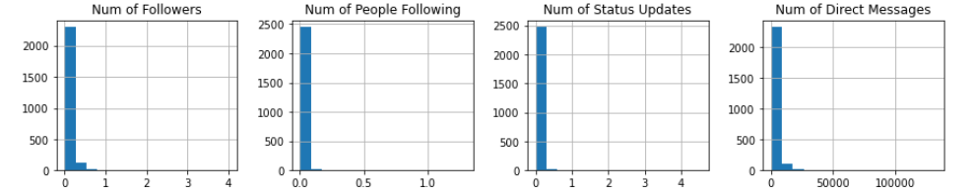
\includegraphics[width=\columnwidth]{skewed.png}
\caption{Distribution of Numerical Features}\label{num_feat_dist}
\end{figure}

\noindent As we can see in Figure \ref{num_feat_dist}, our numerical features are skewed and we used a log transform to make them more normal. See Figure \ref{log_funct}.


\begin{figure}[H]
\centering
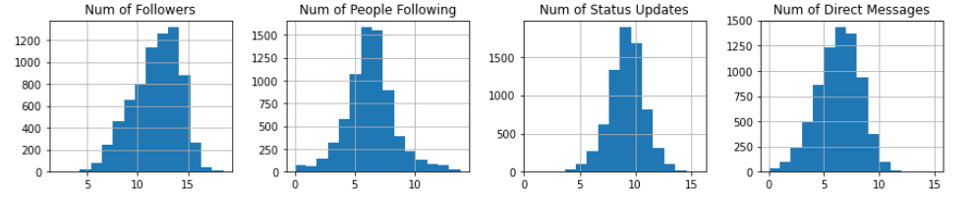
\includegraphics[width=\columnwidth]{normal.png}
\end{figure}

\subsection{Outliers}
There were  many outliers in the dataset. We did an analysis with a boxplot. Given the size of our train dataset (7500 observations), we did not  remove all the outliers. We decided to choose 200,000 likes as a threshold and remove all the data points above it. The reason we chose this number was the fact that our data points are well condensed below 200,000 as can be seen in the next picture. 
\begin{figure}[H]
\centering
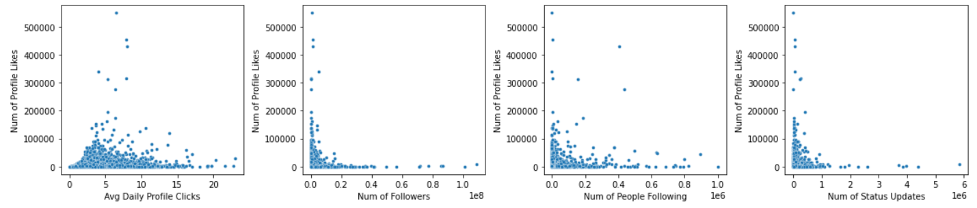
\includegraphics[width=\columnwidth]{scatter.png}
\end{figure}

\subsection{Scaling}
As many machine learning models such as linear models require scaling, we decided to StandardScaler from Sklearn to standardize our data. See Figure \ref{standarization}.

% moved to appendix
% \begin{figure}[H]
% \centering
% 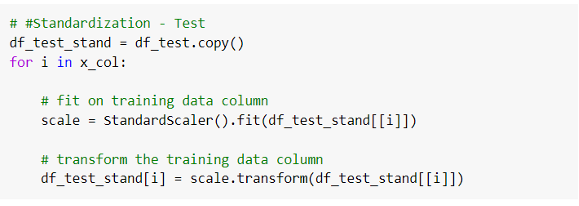
\includegraphics[width=\columnwidth]{standardize.png}
% \end{figure}

\subsection{Feature Selection}
We used the Select K Best algorithm with mutual\_info\_regression for feature selection. Mutual\_info\_regression estimates mutual information for a continuous target variable. Mutual information (MI) between two random variables is a non-negative value, which measures the dependency between the variables. It is equal to zero if and only if two random variables are independent, and higher values mean higher dependency. [Sklearn]

% moved to appendix
% \begin{figure}[H]
% \centering
% 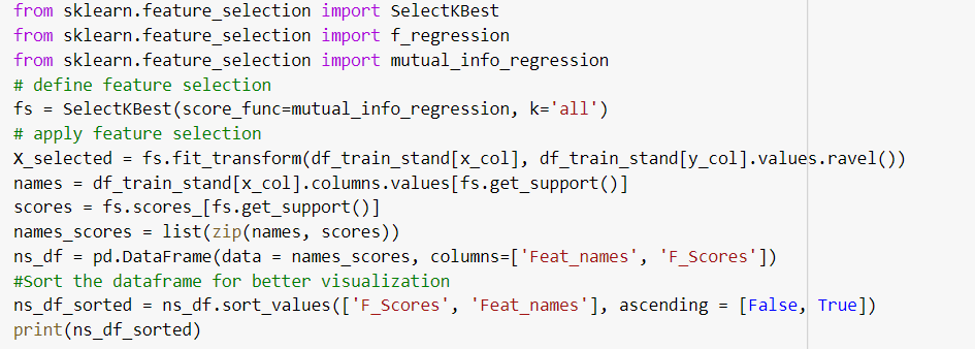
\includegraphics[width=\columnwidth]{selectkbest.png}
% \end{figure}
% \begin{figure}[H]
% \centering
% 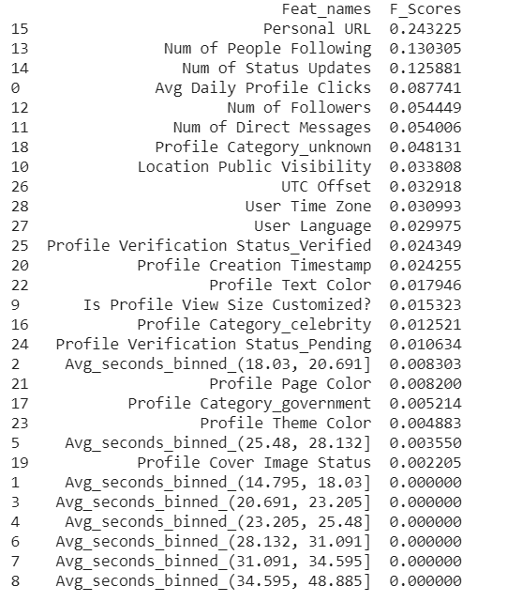
\includegraphics[width=\columnwidth]{features.png}
% \end{figure}
\noindent After that we tried different number of features based on above and finally we used top 21 features for our best results.


\section{Methodology}
As mentioned earlier, we followed an iterative process in which we conceptually embedded a feedback-loop. Data is not a blackbox and the preprocessing can heavily impact the model performance. In this section, we present two different avenues we took in order to develop a model that performs well. A good model is a model that generalizes well on previously unseen data.

\subsection{From linear models to gradient boosting}
We first started by testing linear models which provided decent results.
We then decided to use more complex models - here, gradient boosting.  A model that is more complex should be able to capture more relationships between our features and thus lead to better results.  

\subsubsection{Hyper parameter tuning and cross-validation}
We optimized each model by tuning the hyper parameters using an exhaustive search over a grid of specified values. For each combination of values specified in the grid, we methodically fit the estimator and then evaluated it using 10-fold cross validation (CV). Cross-validation was used as it reduces the variability of the estimate of the test error and tends to not overestimate it too much. 

We split the provided data (discarding the images) into training/test splits of ratio 80/20. CV was applied on the training set split by splitting it further into 10 different folds of approximately equal size. The first fold was treated as the validation set, which was used to evaluate the error after the model had been fit on the remaining 9 folds. We repeated this procedure 10 times and the CV results were simply the average of the error calculated at each iteration. This process was executed for every combination of values in the grid, after which we kept the estimator with the combination that led to the best CV results. Finally, we applied that estimator to the test set split in order to obtain an unbiased estimate of our test error.


% For each estimator, we have followed the same approach. We tuned the hyper parameters using an exhaustive search over a grid of specified values. This approach methodically builds and evaluates the performance of the estimator for each combination of values specified in the grid. More specifically, we use 10-fold cross-validation (CV) in order to evaluate the performance of the estimator for each combination of hyper parameters. Considering the variability and overestimation of the test error in the context of the validation set approach, cross-validation presents the advantage of minimizing these two drawbacks. 
% For our purpose, we split the provided data into training/test sets of ratio 80/20. Cross-validation was then applied on the training set split. The idea is then to split further the training set into 10 different folds of approximately equal size. The first fold is treated as the validation set and the model is fitted on the remaining 9 folds. The error is then evaluated on the held-out validation set and this procedure is repeated 10 times. The results of the 10-fold CV is the average of the error calculated at each iteration. Cross-validation tends to not overestimate the test error too much compared to the validation set approach as it leads to less bias. Our grid search will then provide us the estimator and associated hyper parameters that lead the best CV results. We use that resulting estimator on the held out test set to assess that our estimator does not have too much variance. 

\subsubsection{RMSLE and log-transform}
The metric used as part of the competition to assess the performance of the models was the RMSLE, expressed as follows:
\begin{equation}
    RMSLE = \sqrt{\frac{1}{n}\sum_{i=1}^{n}(\log(p_{i}+1) - \log(t_{i} + 1))^{2}}
\end{equation}
where $p_{i}$ is the predicted value for observation $i$ and $t_{i}$ its true value. Considering we are in a regression analysis setting, some of our predictions might be negative. The RMSLE, which uses the natural logarithm, is not defined for negative values. This is not a problem for the neural network (we will discuss this later) as it uses the $ReLU$ activation function for the hidden layer and a linear one for the ouput layer. The $ReLU$ forces all values to be positive which only leads to positive predictions. However, it constitutes a problem for all the other models for which the output space is not restricted to positive values.

We took care of this problem during training by projecting the values of our target variable onto the log-space as follows:
\begin{equation}
    \hat{t_{i}} = \log(t_{i} + 1)
\end{equation}
where $\hat{t_{i}}$ is the log-transformed target value. We then train our model using the Root Mean Squared Error (RMSE):
\begin{equation}
    RMSE = \sqrt{\frac{1}{n}\sum_{i=1}^{n}(p_{i} - t_{i})^{2}}
\end{equation}
After the training was completed, we approximately reverse-transformed the predicted values to their original scale by applying the natural exponent. If we wanted to perform the exact inverse, we would have needed to subtract one to the result of the exponentiation. However, this could still have led to negative predictions for values really close to 0. Moreover, an empirical analysis showed that the error induced by approximating the inverse was minimal.

\subsubsection{Linear Regression}
The first statistical model we tried was Linear Regression, expressed as follows:
\begin{equation}
    y = f(X) + \epsilon
\end{equation}
where $y \in \mathbf{R^{n}}$ and $X \in \mathbf{R^{n \times p}}$: y is the vector of predicted values, X is the input with n observations and p independent variables. Linear regression assumes that the true relationship between X and Y is linear and that $\epsilon$ is a mean-zero random error term. We can use a residuals plot to verify those assumptions.
\begin{figure}[H]
\centering
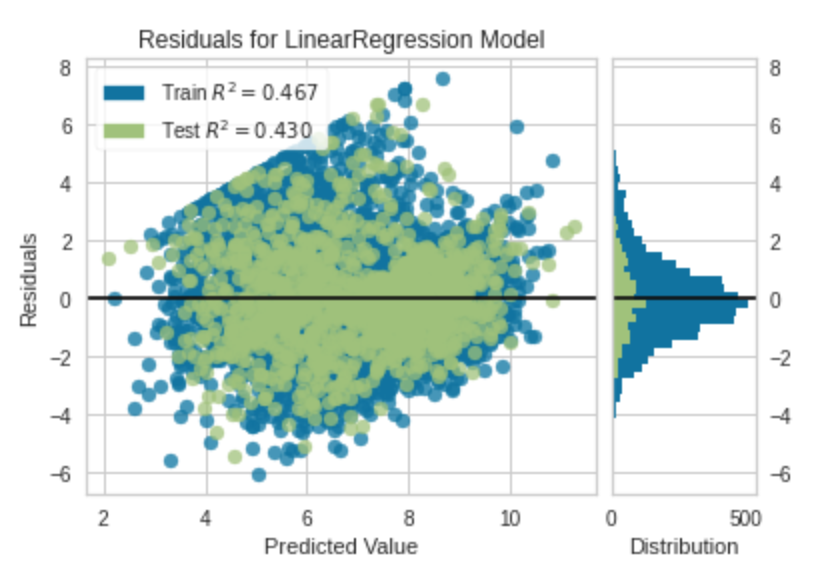
\includegraphics[width=\columnwidth, scale=0.5]{residuals_plot_lr.png}
\caption{Residuals plot for Linear Regression}
\label{residuals}
\end{figure}
As shown in figure \ref{residuals}, the residuals seem to be randomly scattered around the 0 horizontal axis. Furthermore, the right part shows that the distribution of the residuals seems to follow a normal distribution with mean 0. Linear models thus seem appropriate for our training set.
\subsubsection{Regularized linear regression} As we assume that X and y follow a linear relationship, exploring regularized linear models seems like the next logical step. Regularization helps in reducing variance (while introducing some bias) as it favours simpler models. 

The first regularized model is the \textbf{Least Absolute Shrinkage Selector Operator (LASSO)} which assigns a penalty equal to the sum of the absolute values of the coefficients. The particularity of LASSO is that it can shrink some of the coefficients to 0 thus eliminating some features. Another method would be \textbf{Ridge} regression. We also assigned some penalty to the weights of the regression model but the penalty corresponds to the sum of the squared magnitude of the coefficients. Consequently, the coefficients can never shrink to 0 and this method does not eliminate any features. Finally, \textbf{Elastic Net} is a hybrid of both LASSO and Ridge.

\subsubsection{Gradient Boosting}
We then explored models that are more flexible than the ones described previously. We thus turn towards gradient boosting. Similarly to bagging, boosting is an ensemble technique in which we use many "weak" learners - decision trees in our case -  and combine them using some model averaging technique. A weak learner is simply a decision tree that would perform relatively poorly on its own. However, boosting differs from bagging in the sense that the weak learners are not built independently but sequentially. 

Indeed, the intuition is that every subsequent learner learns from the mistakes of the previous ones. Specifically, in the regression analysis setting, we can assume that our goal is to teach a model F that makes predictions of the form $\hat{y} = F(X)$. It does so by minimizing, in an iterative process, a loss function. At every stage $m \in (1,...,M)$, we have a general estimator $F_{m-1}$. The aim is to improve this mode $F_{m-1}$ by fitting a new weak learner $h_{m}$ to the residuals of the previous learners. Therefore, at each stage m, a new estimator is added to the general model in an attempt to correct the errors made by the previous learners. 

Intuitively, we can see gradient boosting as using gradient descent to solve an optimization problem with respect to some loss function.

\subsubsection{XGBoost and Light Gradient Boosting Machine (LightGBM)}
We used two specific implementations of gradient boosting: XGBoost and LightGBM. They mainly differ in the way the decision trees are growing (see figure \ref{tree_growth}). XGBoost applies level-wise tree growth which consists in maintaining balanced trees. On the other hand, LightGBM applies leaf-wise tree growth which splits the leaf that reduces the loss the most. It makes it a more flexible model prone to overfitting.
\begin{figure}[H]
\centering
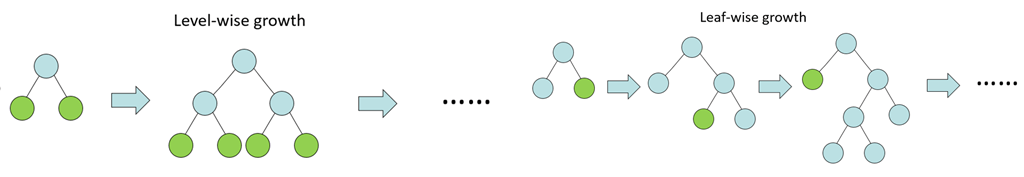
\includegraphics[width=\columnwidth]{leaf_level_wise.png}
\caption{Difference between level-wise and leaf-wise tree growth \cite{keitakurita_2019}}\label{tree_growth}
\end{figure}
\subsubsection{Voting Regression}
Finally, building on the idea that combining multiple estimators and performing a model-averaging technique usually reduces overall variance, we combine XGBoost and LightGBM using a Voting Regression model. This model averages the individual predictions from each of the base models to form the final prediction. We present and discuss the results in the "Results and discussion" section.

\subsection{Neural Network}
We experimented with a deep-learning approach, using variants of a small Neural-Network.  

\subsubsection{Architecture}
The parameters we examined were the number of neurons per layer (the width) and the number of layers (depth). In our design, we calculated the number of neurons as  function of input size. As we experimented with the count of features, this formula represented how many inputs to pass between the layers. $((features*constant))$

We experimented with the depth of our network too. With more layers, we realized we were able to capture more aspects and relationships between the data points.
\subsubsection{Design and Hyperparameters}
We observed high proclivity of the network to overfit. To address this trend, we added two dropout layers and trained on a learning rate schedule. Dropout layers drop a certain percentage of the weights randomly. Effectively, they make the network less sensitive to the specific weights of neurons. This was constructed to decrease memorization between the layers of our network. We trained on a slower learning rate, reducing our model's response to error.

We constructed two structures. These two varied in the number of neurons in their input and hidden layer. The larger of the two is depicted in \ref{neuralnetimage}, with a total of ~7,700 trainable parameters. The smaller model contained ~2400 trainable parameters.

\section{Results and discussion}

\subsection{Linear Models}
\vspace{-3mm}
\begin{table}[H]
\begin{tabular}{|l|l|l|l|l|}
\hline
              & \textbf{Linear Reg.} & \textbf{Lasso}  & \textbf{Ridge}  & \textbf{ElasticNet} \\ \hline
\textbf{CV RMSLE}      & 1.6311      & 1.6979 & 1.6912 & 1.6919     \\ \hline
\textbf{Public score}  & 1.8725      & 1.8733 & 1.8728 & 1.8728     \\ \hline
\textbf{Private score} & 1.7408      & 1.7405 & 1.7411 & 1.7411     \\ \hline
\end{tabular}
\caption{Cross-validation and test results}
\label{tab:linear-models}
 \vspace{-5.8mm}
\end{table}
\vspace*{-\baselineskip}

Table \ref{tab:linear-models} demonstrates that all three models provide very similar results. Lasso, Ridge and ElasticNet did not provide any improvement on Linear Regression. This can be explained in a simple way: linear regression model is too simple for our training data. This means that it did not overfit and our regularized models, whose aim is to reduce overfiting, were not valuable. They optimized regularized models converged towards a simple linear regression model. ElasticNet being a hybrid of Lasso and Ridge, it converged towards the regularized model that gave better results which was Ridge.
\subsection{Gradient boosting and voting regression}
\vspace*{-\baselineskip}
\begin{table}[H]
\begin{tabular}{|l|l|l|l|}
\hline
                       & \textbf{XGBoost} & \textbf{LightGBM} & \textbf{Voting Reg.} \\ \hline
\textbf{CV RMSLE}      & 1.5408           & 1.5413            & 1.5303                    \\ \hline
\textbf{Public score}  & 1.7895           & 1.7723            & 1.7674                    \\ \hline
\textbf{Private score} & 1.6785           & 1.6748            & 1.6719                    \\ \hline
\end{tabular}
\caption{Cross-validation and test results for ensemble}
\label{tab:ensembling}
\end{table}
\vspace*{-\baselineskip}
Table \ref{tab:ensembling} shows that gradient boosting performed better than linear models. XGBoost and LightGBM being more flexible models, they did better capture the inherent relationships between the features. Linear models usually work well in practice but require extensive feature engineering. Our feature engineering led to more than decent scores with linear models. However, considering the nature of gradient boosting algorithms, we reached better scores with the same feature engineering. As we can see in the \ref{tab:ensembling}, using a voting regression combining XGBoost and LightGBM did not provide much improvement. Voting regression usually helps in reducing variance. However, since our models did not present high variance at first, the improvement was minimal.

\subsection{Note on cross-validation results}
As can be seen in table \ref{tab:linear-models} and table \ref{tab:ensembling}, the CV RMSLE tends to underestimate the generalization error. This seems to be contradictory with the definition of CV we previously gave - CV error usually overestimates the test error. However, this observation is explained by the fact that our models are cross-validated using the RMSE rather than the RMSLE. Indeed, we log-transform our target values before fitting our models. The RMSE is thus evaluated using the predictions on the log-space which explains why we see lower CV error.

\subsection{Neural Network Approach}
In validating our Neural Networks, we used cross-validation.  We captured the full spread of data and utilize all of our limited data. Our best result on the private dataset was a RMSLE of 1.6712.

However, we recognize shortcomings with this approach. As observed on table \ref{tab:nn}, our approach underestimated the model's performance. We overestimated the training and validation error. Additionally, we recognize the limited scale of this approach. With a larger dataset or model, the  training time would be cumbersome and computationally-intensive.

\begin{table}[H]
\begin{tabular}{|l|l|l|l|}
\hline
                       & \textbf{5-layer: 7000} &  \textbf{5-layer: 1200}\\ \hline
\textbf{CV RMSLE}      & 1.8601     &         1.8490             \\ \hline
\textbf{Public score}  & 1.80226    &         1.80696           \\ \hline
\textbf{Private score} & 1.6712      &        1.67770              \\ \hline
\end{tabular}
\caption{Cross-validation and test results for the 5-layer Neural-Network}
\label{tab:nn}
\end{table}

\vspace*{-\baselineskip}

\section{Conclusion}
In completing this project, we realized the value of data exploration and feature extraction. While there are different strategies to develop a well-generalizing model, the core element was the data.  For example, applying a logarithmic transform on the data increased our performance. We see great value in understanding our input well before passing it to the next stage of a Machine or Deep learning pipeline.

% \section{Citations and Bibliographies}

% The use of \BibTeX\ for the preparation and formatting of one's
% references is strongly recommended. Authors' names should be complete
% --- use full first names (``Donald E. Knuth'') not initials
% (``D. E. Knuth'') --- and the salient identifying features of a
% reference should be included: title, year, volume, number, pages,
% article DOI, etc.

% The bibliography is included in your source document with these two
% commands, placed just before the \verb|\end{document}| command:
% \begin{verbatim}
%   \bibliographystyle{ACM-Reference-Format}
%   \bibliography{bibfile}
% \end{verbatim}
% where ``\verb|bibfile|'' is the name, without the ``\verb|.bib|''
% suffix, of the \BibTeX\ file.

% Citations and references are numbered by default. A small number of
% ACM publications have citations and references formatted in the
% ``author year'' style; for these exceptions, please include this
% command in the {\bfseries preamble} (before the command
% ``\verb|\begin{document}|'') of your \LaTeX\ source:
% \begin{verbatim}
%   \citestyle{acmauthoryear}
% \end{verbatim}

%   Some examples.  A paginated journal article \cite{Abril07}, an
%   enumerated journal article \cite{Cohen07}, a reference to an entire
%   issue \cite{JCohen96}, a monograph (whole book) \cite{Kosiur01}, a
%   monograph/whole book in a series (see 2a in spec. document)
%   \cite{Harel79}, a divisible-book such as an anthology or compilation
%   \cite{Editor00} followed by the same example, however we only output
%   the series if the volume number is given \cite{Editor00a} (so
%   Editor00a's series should NOT be present since it has no vol. no.),
%   a chapter in a divisible book \cite{Spector90}, a chapter in a
%   divisible book in a series \cite{Douglass98}, a multi-volume work as
%   book \cite{Knuth97}, a couple of articles in a proceedings (of a
%   conference, symposium, workshop for example) (paginated proceedings
%   article) \cite{Andler79, Hagerup1993}, a proceedings article with
%   all possible elements \cite{Smith10}, an example of an enumerated
%   proceedings article \cite{VanGundy07}, an informally published work
%   \cite{Harel78}, a couple of preprints \cite{Bornmann2019,
%     AnzarootPBM14}, a doctoral dissertation \cite{Clarkson85}, a
%   master's thesis: \cite{anisi03}, an online document / world wide web
%   resource \cite{Thornburg01, Ablamowicz07, Poker06}, a video game
%   (Case 1) \cite{Obama08} and (Case 2) \cite{Novak03} and \cite{Lee05}
%   and (Case 3) a patent \cite{JoeScientist001}, work accepted for
%   publication \cite{rous08}, 'YYYYb'-test for prolific author
%   \cite{SaeediMEJ10} and \cite{SaeediJETC10}. Other cites might
%   contain 'duplicate' DOI and URLs (some SIAM articles)
%   \cite{Kirschmer:2010:AEI:1958016.1958018}. Boris / Barbara Beeton:
%   multi-volume works as books \cite{MR781536} and \cite{MR781537}. A
%   couple of citations with DOIs:
%   \cite{2004:ITE:1009386.1010128,Kirschmer:2010:AEI:1958016.1958018}. Online
%   citations: \cite{TUGInstmem, Thornburg01, CTANacmart}. Artifacts:
%   \cite{R} and \cite{UMassCitations}.

\section{Acknowledgments}
Shoutout to sklearn and keras! 


% \section{Appendices}

% \begin{figure}[H]
% \centering
% 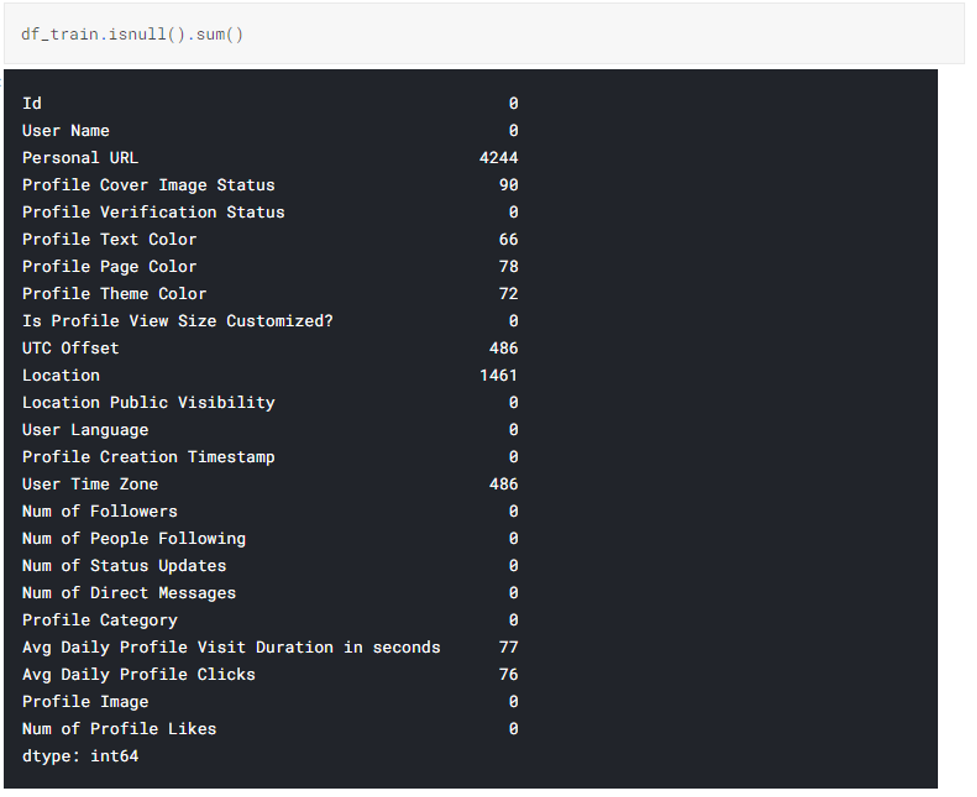
\includegraphics[width=\columnwidth]{Picture1.png}
% \caption{Addressing Missing Values}\label{addressing_missing_values}
% \end{figure}
% %% unique values
% \begin{figure}[H]
% \centering
% 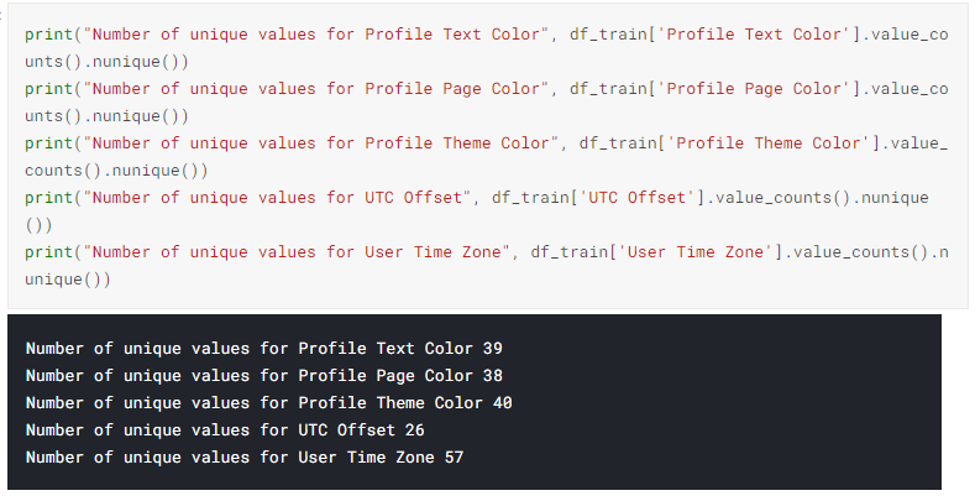
\includegraphics[width=\columnwidth]{Unique values.png}
% \caption{Categorical Unique Values}\label{unique_values}
% \end{figure}

% %% Frequency encoding
% \begin{figure}[H]
% \centering
% 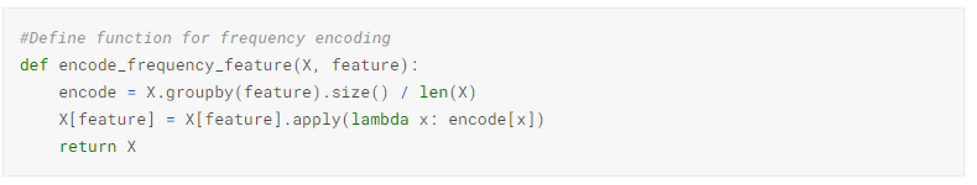
\includegraphics[width=\columnwidth]{Freq enc.png}
% \caption{Frequency Encoding}\label{frequency_encoding}
% \end{figure}

% %% log function 
% \begin{figure}[H]
% \centering
% 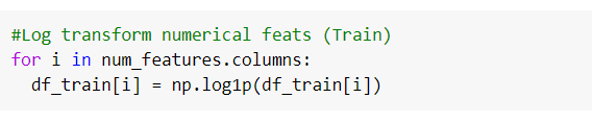
\includegraphics[width=\columnwidth]{log.png}
% \caption{Log Function} \label{log_funct}
% \end{figure}

% %% SELECT K BEST

% \begin{figure}[H]
% \centering
% 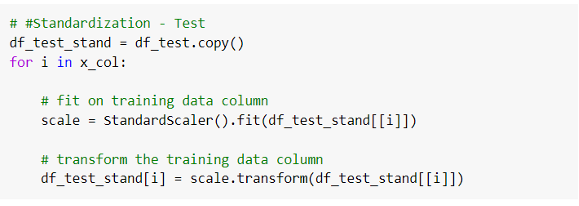
\includegraphics[width=\columnwidth]{standardize.png}
% \caption{Standardize Segment}\label{standarization}
% \end{figure}


% \begin{figure}[H]
% \centering
% 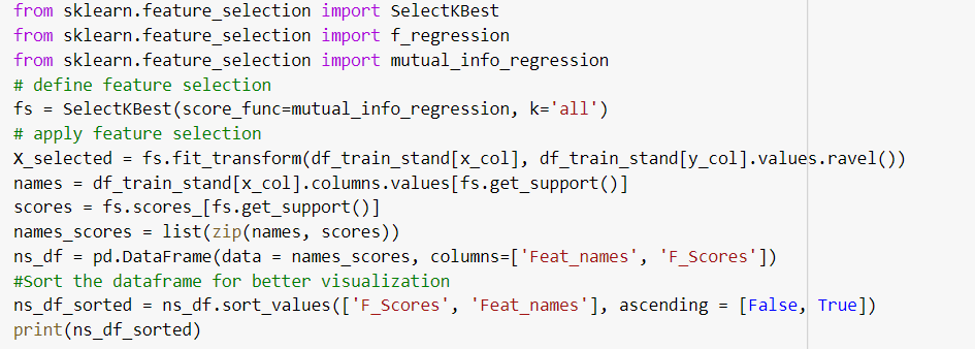
\includegraphics[width=\columnwidth]{selectkbest.png}
% \caption{Select K best features}\label{select_k_best}
% \end{figure}
% \begin{figure}[H]
% \centering
% 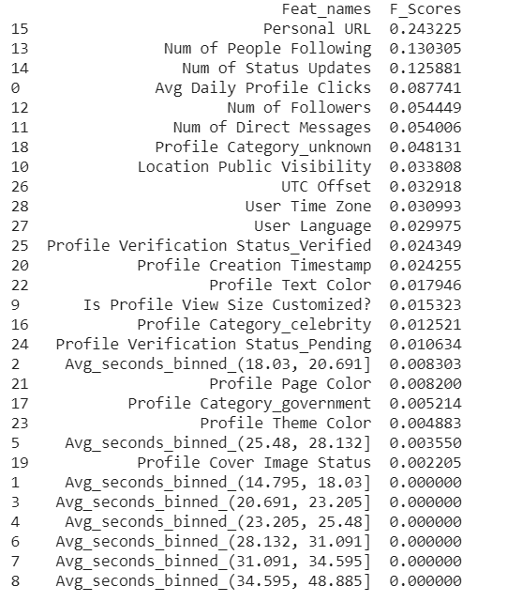
\includegraphics[width=\columnwidth]{features.png}
% \caption{Select K best features output}\label{select_k_best_output}
% \end{figure}


% \begin{figure}[H]
% \centering
% 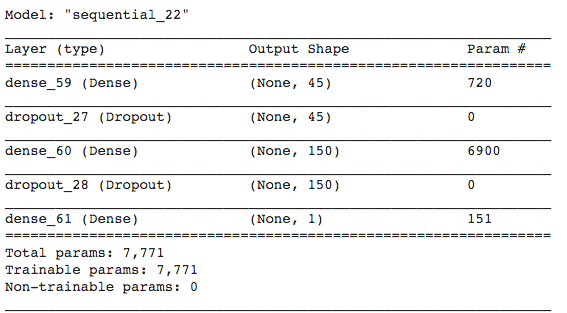
\includegraphics[width=\columnwidth, scale=0.6]{nn_structure.png}
% \caption{Larger Neural Network}\label{neuralnetimage}
% \end{figure}

%%
%% The next two lines define the bibliography style to be used, and
%% the bibliography file.



\bibliographystyle{ACM-Reference-Format}
\bibliography{sample-base}

%%
%% If your work has an appendix, this is the place to put it.
\appendix

\section{Appendix A}
\begin{figure}[H]
\centering
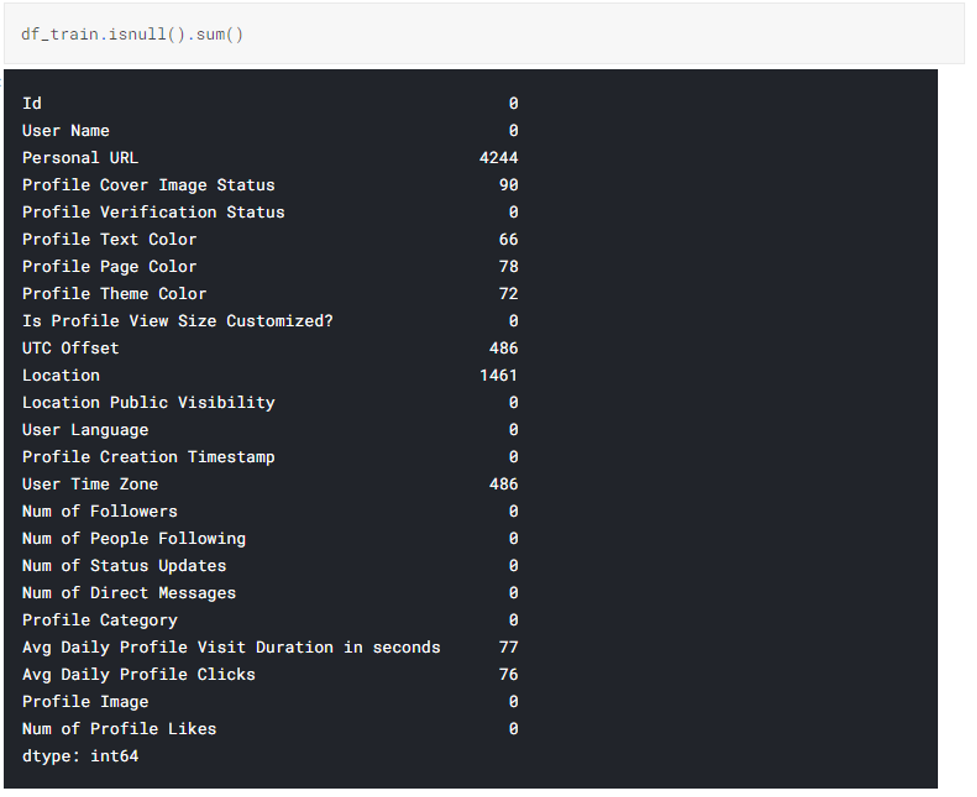
\includegraphics[width=\columnwidth]{Picture1.png}
\caption{Addressing Missing Values}\label{addressing_missing_values}
\end{figure}
%% unique values
\begin{figure}[H]
\centering
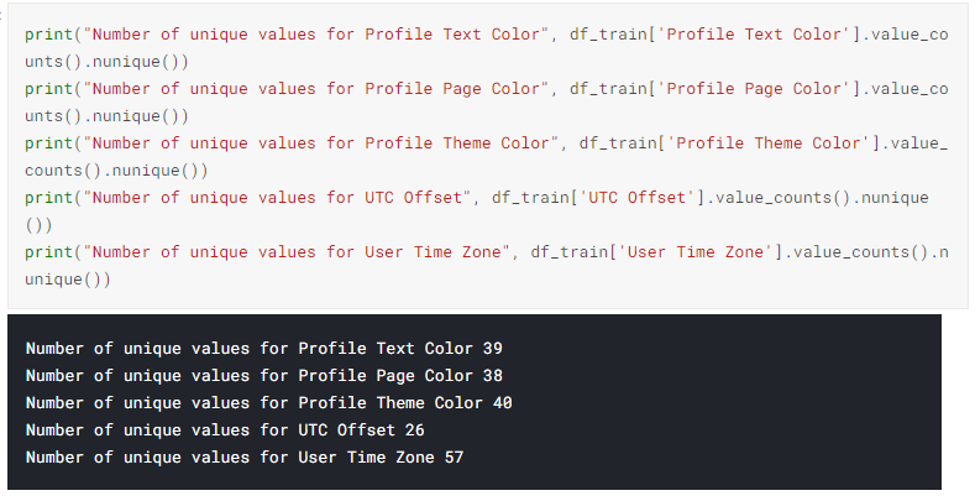
\includegraphics[width=\columnwidth]{Unique values.png}
\caption{Categorical Unique Values}\label{unique_values}
\end{figure}

%% Frequency encoding
\begin{figure}[H]
\centering
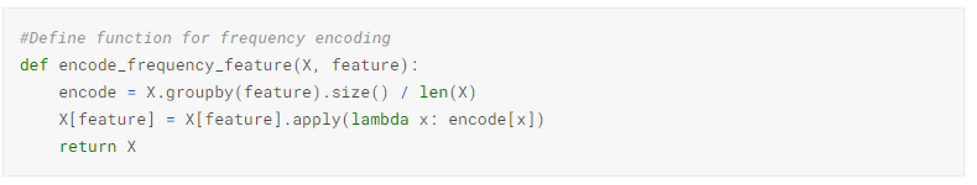
\includegraphics[width=\columnwidth]{Freq enc.png}
\caption{Frequency Encoding}\label{frequency_encoding}
\end{figure}

%% log function 
\begin{figure}[H]
\centering
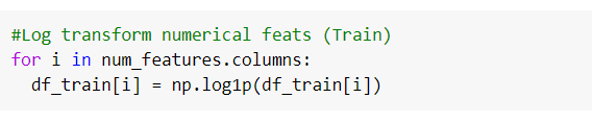
\includegraphics[width=\columnwidth]{log.png}
\caption{Log Function} \label{log_funct}
\end{figure}

%% SELECT K BEST

\begin{figure}[H]
\centering
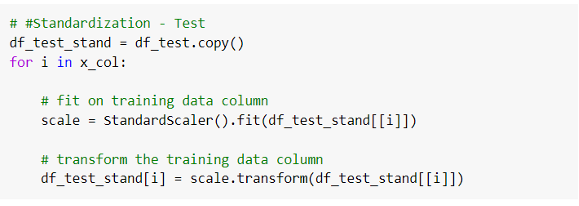
\includegraphics[width=\columnwidth]{standardize.png}
\caption{Standardize Segment}\label{standarization}
\end{figure}


\begin{figure}[H]
\centering
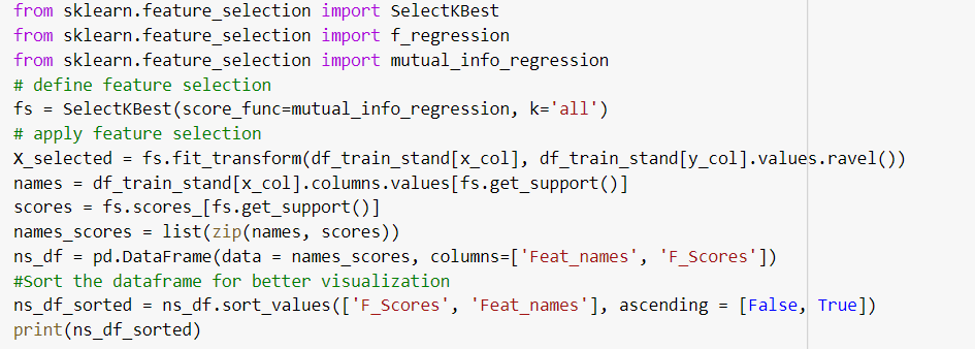
\includegraphics[width=\columnwidth]{selectkbest.png}
\caption{Select K best features}\label{select_k_best}
\end{figure}
\begin{figure}[H]
\centering
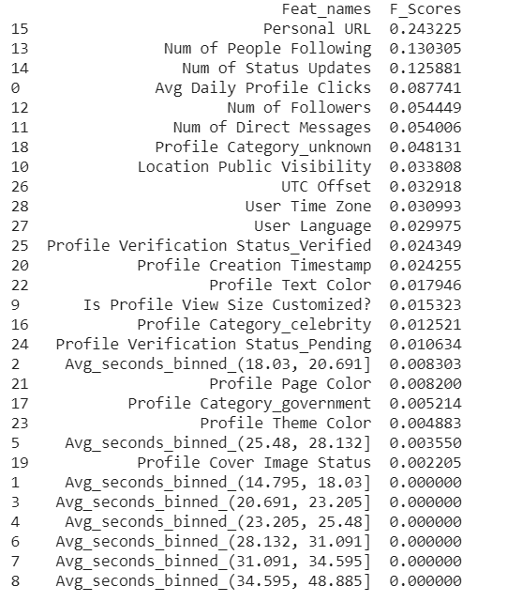
\includegraphics[width=\columnwidth]{features.png}
\caption{Select K best features output}\label{select_k_best_output}
\end{figure}


\begin{figure}[H]
\centering
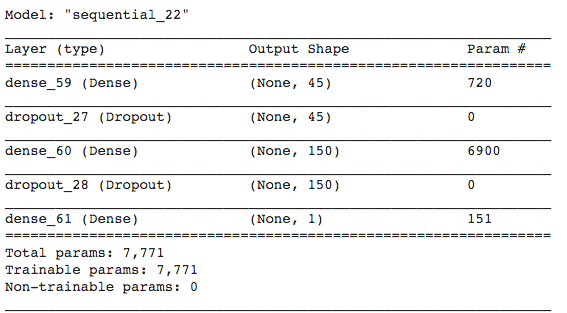
\includegraphics[width=\columnwidth, scale=0.6]{nn_structure.png}
\caption{Larger Neural Network}\label{neuralnetimage}
\end{figure}

% \section{Appendix A}

\end{document}
\endinput
%%
%% End of file `sample-sigplan.tex'.
